\documentclass[pidr]{tnreport}
%\documentclass[confidential,pidr]{tnreport} % If you are writing confidential report

\def\reportTitle{DynGraph : Logiciel de dessins et d'édition de graphes} % Titre du mémoire
\def\reportLongTitle{DynGraph : Logiciel de dessins et d'édition de graphes} % Titre plus long du mémoire

\def\reportAuthor{Jean-Baptiste Dominguez\\ Raphael Moulet}
\def\reportAuthorEmail{\email{jean-baptiste.dominguez@telecomnancy.eu}\\ \email{raphael.moulet@telecomnancy.eu}} % Courriel de l'élève

\def\reportSupervisor{Christophe Simon} % Prénom Nom de l'encadrant industriel
\def\reportCompany{CRAN} % Nom de l'entreprise d'accueil
\def\reportCompanyAddress{Campus Sciences, Boulevard des Aiguillettes, BP 70239}  % Adresse de l'entreprise
\def\reportCompanyCity{54506, VANDOEUVRE-LES-NANCY} % Adresse (cont.) de l'entreprise
\def\reportCompanyPhone{06 51 40 08 01} % Téléphone de l'entreprise
\def\reportCompanyLogoPath{figures/logo/logo_cran} % Logo de l'entreprise -- comment this definition to remove company logo

\def\reportProjectLogoPath{figures/logo_project}

\def\place{Villers-les-Nancy} % Ville pour la signature pour l'engagement anti-plagiat
\def\date{\today} % Date pour la signature de l'engagement anti-plagiat

\def\reportProjectCustomer{Projet réalisé pour l'équipe du CRAN}

\begin{document}
  
\maketitle
\pagenumbering{roman}

\insertAntiPlagiarismAgreement{Dominguez, Jean-Baptiste}{31418117}
\insertAntiPlagiarismAgreement{Moulet, Raphael}{31415907}

\cleardoublepage

\makesecondtitle

\section*{Remerciements}
\addcontentsline{toc}{chapter}{Remerciements}

{\em
``Nous tenons à remercier notre encadrant Christophe Simon pour le temps accordé et consacré. Il nous a permis de visualiser l'ampleur du projet et son utilisation au quotidien.\\
Nous remercions également l'école "Télécom Nancy" qui nous a permis de rendre cela possible.``
}

\hspace{4cm} -- L'équipe DynGraph


\cleardoublepage

\renewcommand{\baselinestretch}{0.5}\normalsize
\tableofcontents
\renewcommand{\baselinestretch}{1.0}\normalsize
\cleardoublepage

\pagenumbering{arabic}
\setcounter{page}{1}

\chapter{Introduction}

L’analyse de graphe est primordiale en recherche puisque de nombreux systèmes - réseaux, villes, infrastructures et liens de toutes natures - peuvent être représentés par des graphes.
Or les chercheurs ne sont pas satisfaits : 

\begin{itemize}
\item les logiciels existants d’édition de graphe ne possédaient pas toutes les fonctionnalités recherchées
\item aucun n’utilise Matlab et les variables de son workspace, alors qu’il est très répandu dans le milieu. Notre encadrant souhaite un programme qui met ces variables à jour  de manière à pouvoir sauvegarder un graphe et le réutiliser ou le communiquer
\end{itemize}

L’objectif est donc de créer un environnement d’édition et de manipulation de graphe dans Matlab.

Pour obtenir un logiciel correspondant à son besoin et celui de ces collègues, M. Christophe Simon a envoyé un sujet de PIDR à Télécom Nancy. N’étant pas satisfait du résultat du groupe de 2015, il relance en 2016, et l’équipe composée de Raphaël Moulet et Jean-Baptiste Dominguez choisit ce sujet.

Au fil de réunions régulières entre encadrant et élèves ingénieurs, le cahier des charges est rempli et le logiciel DynGraph Editor for Matlab est développé.

Nous exposerons tout d’abord les besoins et contraintes du cahier des charges, puis l’organisation, la réalisation et la présentation de notre application avant de conclure.

\cleardoublepage

\chapter{Présentation du projet}

\section{Analyse des besoins}

La situation de départ était celle d’une absence de logiciel répondant à un besoin spécifique. Nous avons créé un logiciel de bout en bout.

\subsection{Environnement de travail}

Utilisation de Matlab : 

\begin{itemize}
\item le programme devra se lancer à partir de lignes de commandes matlab
\item il utilisera des variables d’une classe spécifiquement développée pour  ce programme
\item cette classe devra définir une structure pour les graphes utilisés
\item il comportera une interface graphique permettant l’édition du graphe
\item l’édition graphique du graphe devra modifier la variable dans le workspace en temps réel
\item il sera possible de charger des graphes déjà remplis et partager des graphes entre utilisateurs
\end{itemize}

Langage informatique :

\begin{itemize}
\item à part la classe matlab, le langage à utiliser est laissé au choix des développeurs
\item le programme ne devra pas être à part de matlab - il doit y être intégré. Par exemple, le lancer n’ouvrira pas un autre programme mais une fenêtre dans matlab et fermer matlab fermera donc le programme
\end{itemize}


\subsection{Edition de graphes}

L’objectif est de pouvoir représenter les différents types de graphes : 

\begin{itemize}
\item graphes orientés
\item p-graphes
\item graphes colorés
\end{itemize}

Gestion des noeuds et arcs : 

\begin{itemize}
\item il sera possible d’ajouter et supprimer des noeuds et des arcs, ainsi que de les éditer
\item il sera possible de déplacer les noeuds
\item les noeuds devront posséder un nom, qui pourra être édité
\item les arcs devront posséder une couleur et une direction. La direction devra être indiquée par une flèche et les couleurs suffisamment distinctes.
\item les arcs ne doivent pas avoir de poids, ceci est inutile dans le domaine d’utilisation
\item la configuration graphique devra pouvoir être sauvegardée
\item il sera possible d’avoir plusieurs arcs entre deux noeuds, ainsi que des arcs ayant le même noeud comme origine et fin. Ces arcs ne devront pas se superposer
\end{itemize}

\subsection{Utilisation}

Pour les utilisateurs:
\begin{itemize}
\item le programme devra pouvoir être installé sur des versions de matlab plus ou moins récentes. Des directives d’installation devront être fournies
\item le programme devra être facile à prendre en main. Une documentation bien remplie sera à disposition des utilisateurs
\item si possible, il serait utile de faire un zoom et se déplacer dans la fiche
\end{itemize}

Pour les développeurs:
commenter le code de manière à ce que d’autres équipes puissent comprendre son fonctionnement et éventuellement ajouter des fonctionnalités

\cleardoublepage

\chapter{Organisation}

\section{Méthodes de travail}

Dans un premier temps, nous avons décidé de nous attribuer des rôles : Jean-Baptiste Dominguez, Chef de projet et Raphael Moulet, développeur. Afin de mener à bien se projet, nous avons décidé de nous réunir régulièrement afin de faire le point sur les tâches faites ou restantes à faire. Cela nous a permis d’avoir une certaine agilité dans le développement de notre projet.

\begin{figure}[h]
  \centering
  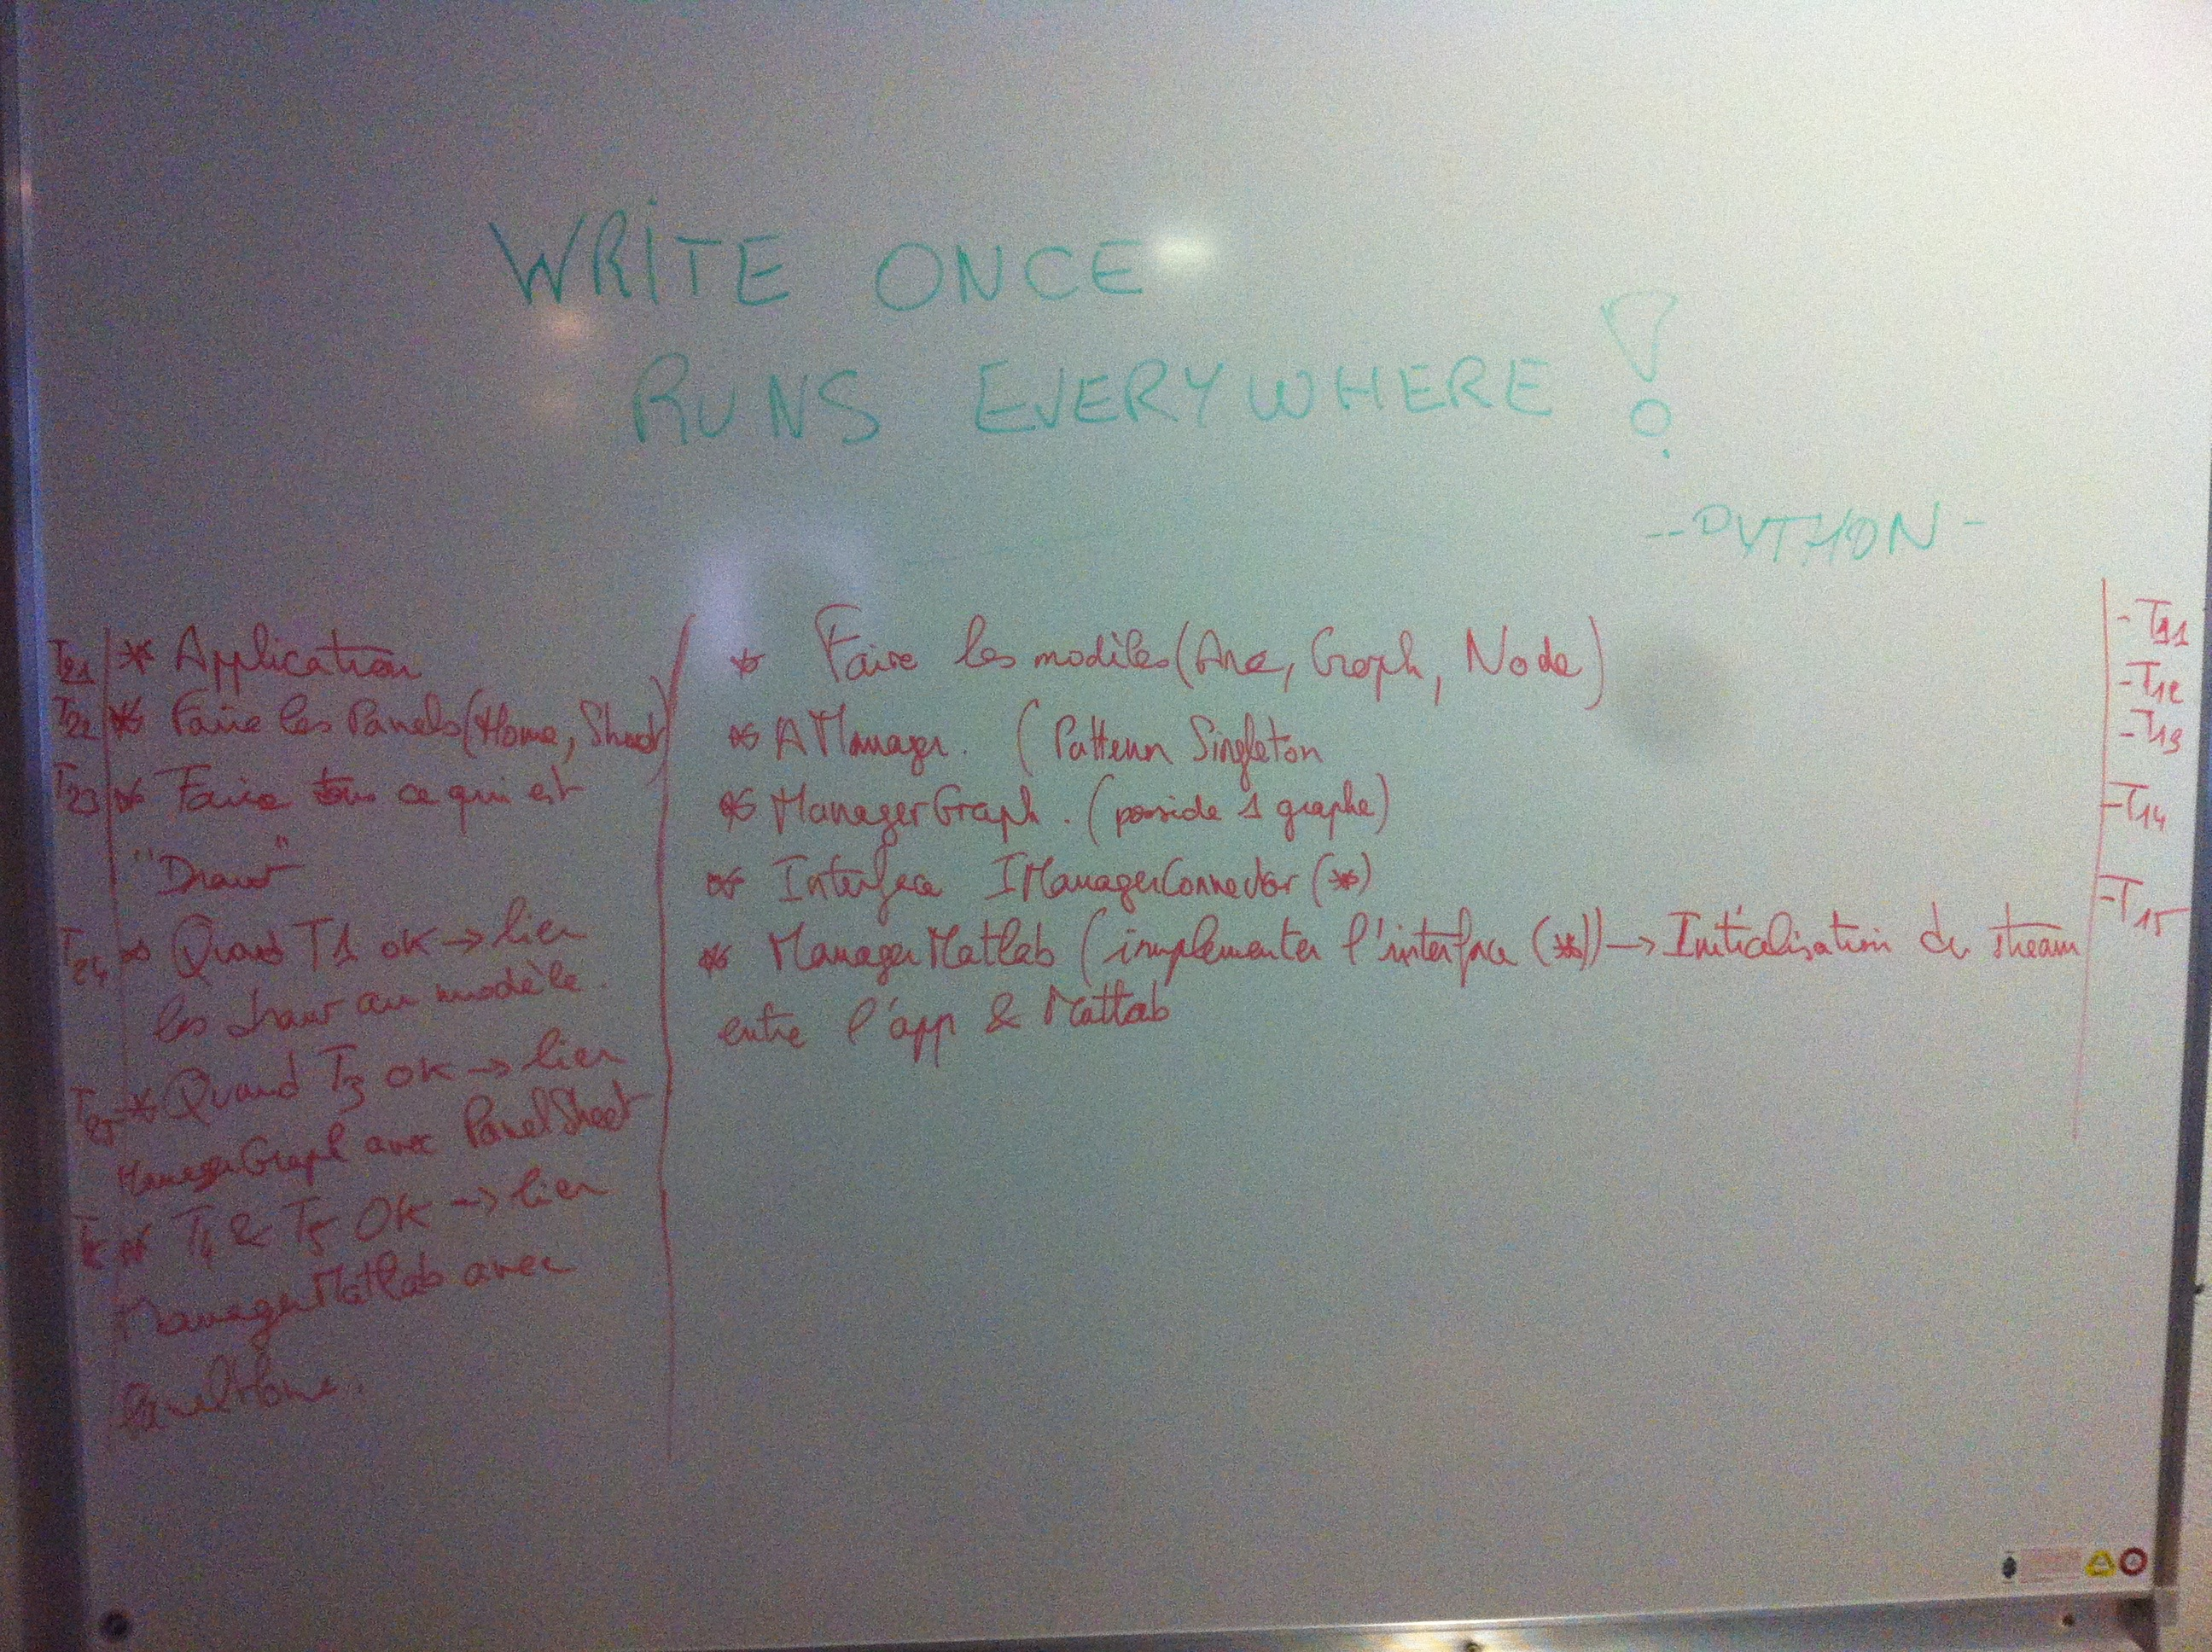
\includegraphics[width=10cm]{figures/tableau}
  \caption{Tableau}
  \label{fig:tableau}
\end{figure}

Nous avons utilisé régulièrement des tableaux et d’autres supports comme des diagrammes de gant afin de faire le point et planifier les prochaines étapes du projet. Nous avions des réunions régulières avec notre encadrant. Grâce à notre découpage des tâches donc à notre agilité, nous avons pu réagir très rapidement à ces remarques et/ou propositions.


\section{Répartition du travail et des tâches, planning}

Nous avons utilisé le logiciel “GranttProject” dans le but de mettre sur logiciel la planification de nos différentes tâches. Nous avons saisi les ressources comme vu sur la figure~\ref{fig:gantt_ressources} ainsi que les tâches générales du projet.

\begin{figure}[h]
  \centering
  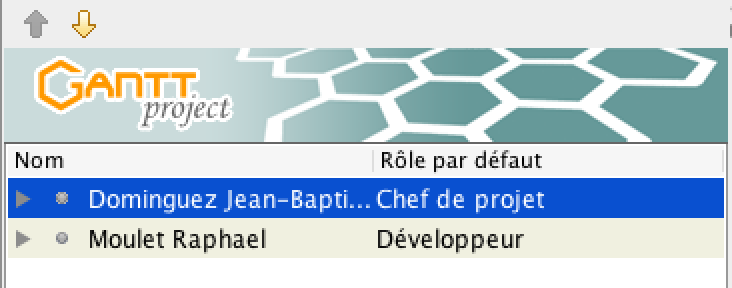
\includegraphics[width=10cm]{figures/gantt_ressources}
  \caption{Les ressources sur GanttProject}
  \label{fig:gantt_ressources}
\end{figure}

Nous avons suivi l’avancement de notre projet par le biais de ce diagramme exposé sur la figure~\ref{fig:gantt_taches}.

\begin{figure}[h]
  \centering
  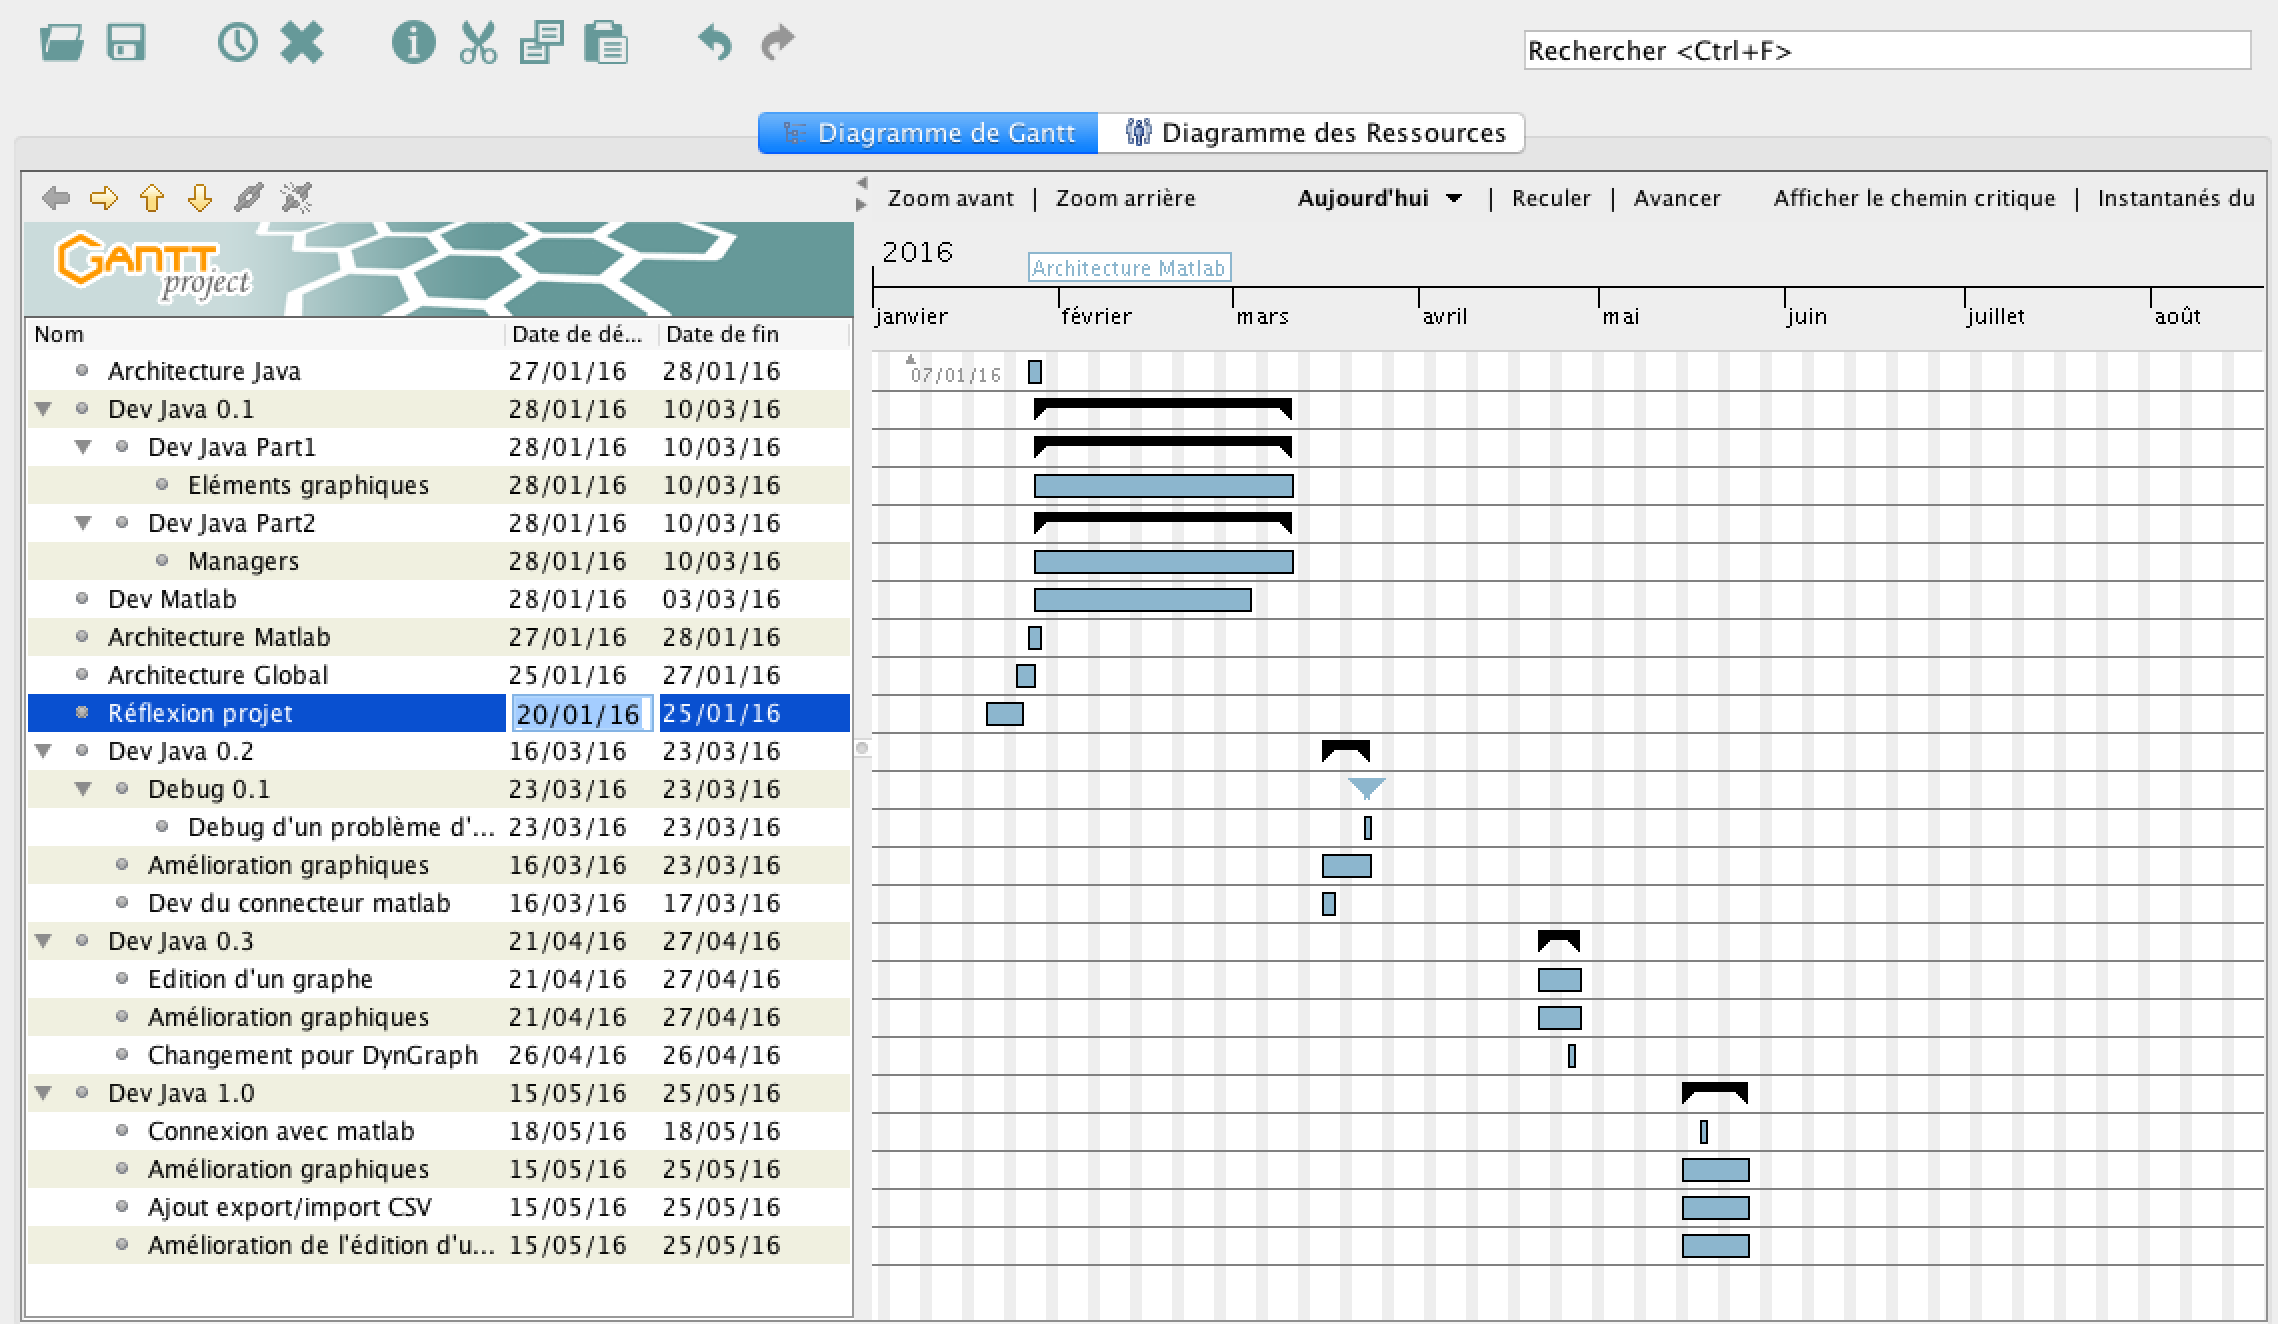
\includegraphics[width=17cm]{figures/gantt_taches}
  \caption{Diagramme de Gant sur GanttProject}
  \label{fig:gantt_taches}
\end{figure}

\cleardoublepage

\chapter{Réalisation de l'application : DynGraph}

\section{Architecture}

Il est possible, à partir de Matlab, de lancer une application java. Suite à la découverte d’une librairie, “matlabcontrol”, permettant la communication entre un programme java et Matlab, nous avons opté pour une logiciel Java lancé depuis notre programme Matlab pour répondre au problème posé. Le choix du langage permettra à un grand nombre de développeurs de pouvoir le maintenir et l’améliorer suite à l’étendu de ce langage dans le monde des développeurs.

Nous utilisons la bibliothèque swing dans laquelle sera gérée la partie graphique. Avec “matlabcontrol”, il est possible de faire des commandes Matlab à partir du code java, ainsi les données seront récupérées directement dans le workspace qui sera modifié en temps réel pendant les manipulations. Voici un récapitulatif de l’architecture de notre application dans la figure~\ref{fig:architecture_global}.

\begin{figure}[h]
  \centering
  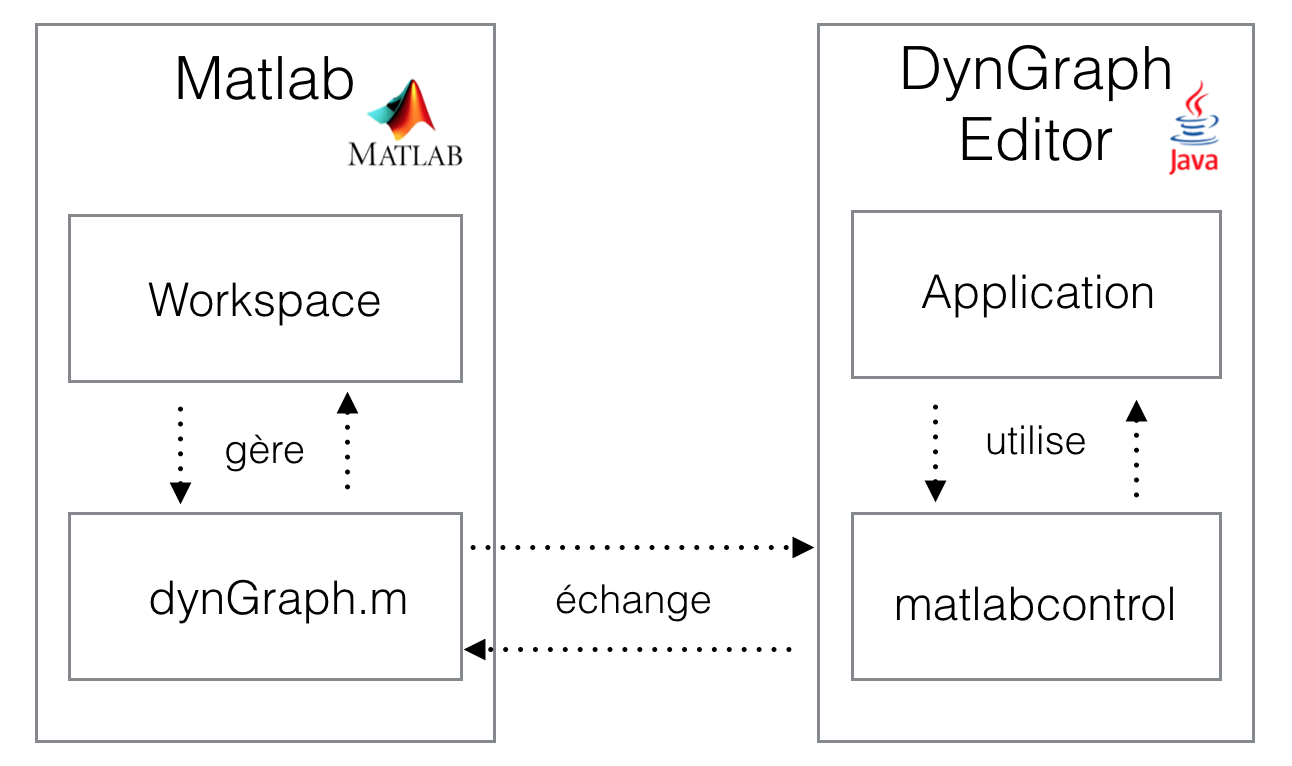
\includegraphics[width=15cm]{figures/architecture_global}
  \caption{Architecture globale}
  \label{fig:architecture_global}
\end{figure}

Pour gérer les données matlab, nous avons décidé de créer une classe matlab appelée “dynGraph” possédant la structure de données présenté ci-dessous avec la figure x.X. Elle nous permet de gérer les données d’un graphe et le lancement de notre logiciel d’édition de graphe par la lecture d’un “.JAR”. La liaison entre matlab et le code java était gérée par une classe appelée ManagerMatlab qui contient les méthodes pour mettre à jour les données dans le workspace lorsque le graphe java est modifié.

Nous avons du définir une structure de données pour gérer un graphe dans notre classe dynGraph. Nous avons 2 types d’objet :
Sommet : ID, nom.
Arc : ID, Sdébut, Sfin, dirigé, couleur.

Dans la classe “dynGraph”, nous avons deux attributs :
La liste des sommets :  [S1, …,Sn]
La liste des arcs : [A1, …,An]

On a des méthodes dans notre classe Matlab “dynGraph” pour créer les différents arcs et noeuds.

Voici une représentation visuelle d’une liste d’arcs qui est sous forme matricielle dans notre classe “dynGraph” sous Matlab sur cette figure~\ref{fig:tableau_liste_arcs} : 

\begin{figure}[h]
  \centering
  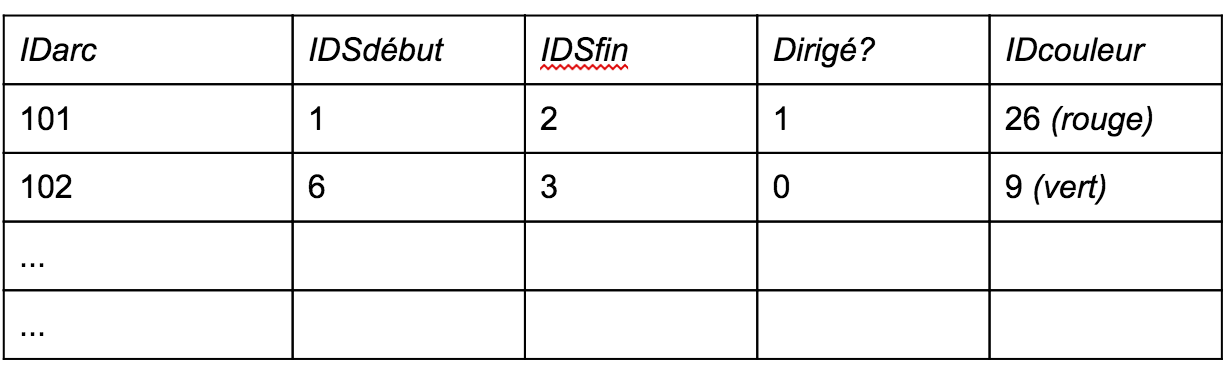
\includegraphics[width=15cm]{figures/tableau_liste_arcs}
  \caption{Tableau d'un liste d'arcs}
  \label{fig:tableau_liste_arcs}
\end{figure}

Le diagramme de classe de la figure~\ref{fig:dc_1} permet de résumer l’architecture de l’application Java.
Comme nous pouvons le remarquer, nous avons une interface "IManagerConnector" qui nous permettrait à l'avenir d'étendre la portabilité de notre application vers d'autres logiciels type Matlab.

\begin{figure}[h]
  \centering
  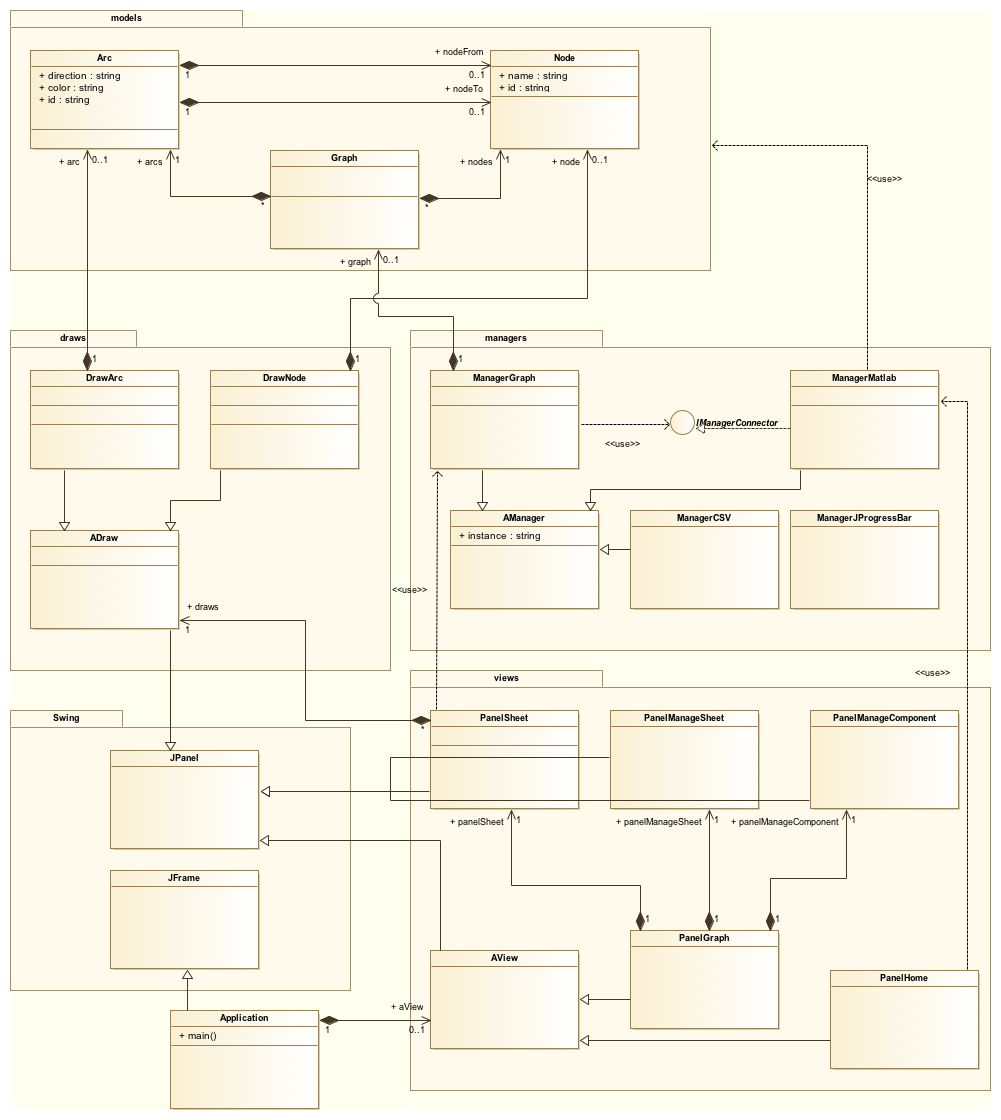
\includegraphics[width=17cm]{figures/dc_1}
  \caption{Diagramme de classe de DynGraph Editor}
  \label{fig:dc_1}
\end{figure}

\clearpage

\section{Présentation de l'application}

\subsection{Partie Matlab}

Nous avons créé la classe dynGraph.m qui permets de gérer des graphes avec la structure définie. C’est une classe de type handle : elle mets automatiquement à jour les graphes qui appellent ses fonctions. 
Le code se trouve en annexe.
Un objet dynGraph est composé d’un vecteur Nodes (noeuds) et d’une matrice Arcs.
La classe est commentée en détail pour son utilisation.
Les méthodes de cette classe sont:

\begin{itemize}
\item draw (name) : lance l’application et dessine le graphe dont le nom est passé en paramètre (et non pas celui appelant la fonction - ce n’est pas intuitif mais ça marche)
\item addNode(nodeID) : ajoute un noeud ou plusieurs, à condition qu’aucun des ID des noeuds ne soit déjà dans Nodes
\item removeNode(nodeID) : enlève un noeud ou plusieurs, à condition qu’ils soient tous contenus dans Nodes. Enlève les arcs liés à ce noeud
\item addArc(arcID, nodeID1, nodeID2, directed, colorID): ajoute un ou plusieurs arcs avec les paramètres précisés. On peut lui passer 3 paramètres minimum - par défaut l’arc n’est pas dirigé et la couleur est 0. arcID est unique
\item removeArc(arcID) : enlève un ou plusieurs arcs
\end{itemize}

Non utilisées par notre programme:

\begin{itemize}
\item addArcs(arcMatrix,  nbArcs) : ajoute des arcs à partir d’une matrice d’arcs suivant notre structure
\item extract() : renvoie Nodes et Arcs
\item clearArcs() et clearNodes(), clearAll()  : vide Nodes et/ou Arcs
\end{itemize}


Nous notons que la classe Java ManagerMatlab contient exactement les mêmes fonctions.

\subsection{Partie Java}

Nous pouvons voir dans la figure~\ref{fig:programme_1} la segmentation des différentes parties de l'application. La partie 1 est continuée d'un menu permettant de changer le nom du graphe ou de modifier une couleur mais également de faire des Import/Export au format CSV.

\begin{figure}[h]
  \centering
  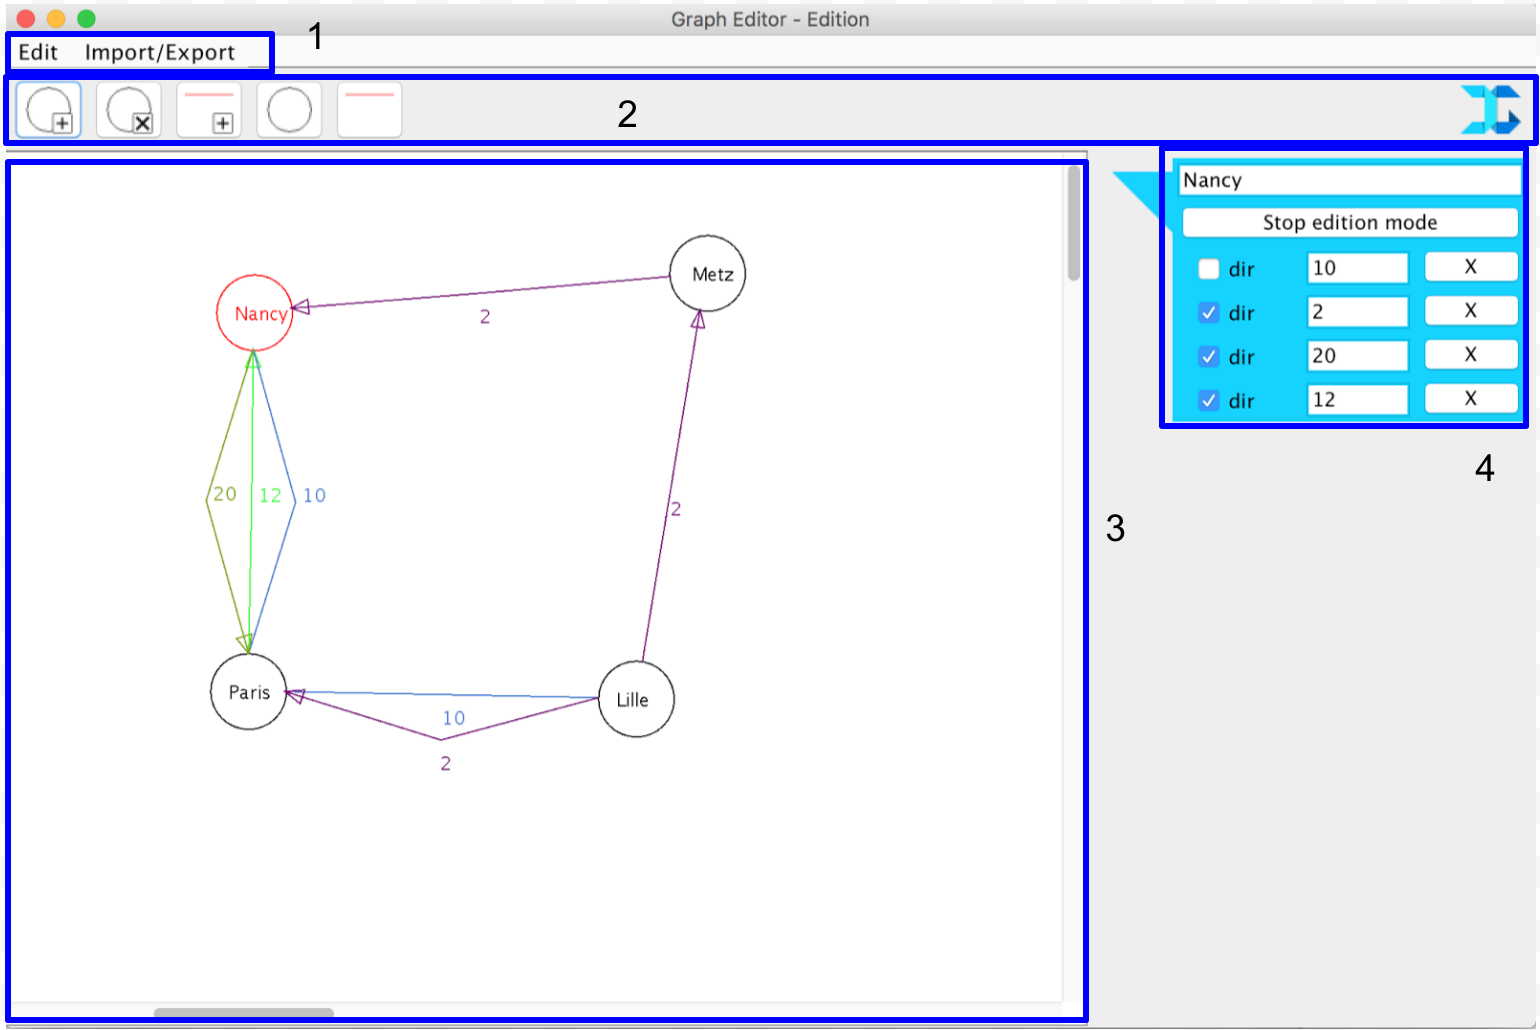
\includegraphics[width=17cm]{figures/programme_1}
  \caption{Ecran de l'application}
  \label{fig:programme_1}
\end{figure}

La partie 2 est un deuxième menu permettant d'interagir avec le menu. C'est le "PanelManageSheet" du diagramme de classe présent dans la figure~\ref{fig:dc_1}. La partie 3 est une feuille gérée par "PanelSheet" où sont placés tous les noeuds et arcs ("DrawNode" \& "DrawArc"). Cette feuille peut être géré par la partie 2. Si nous cliquons sur un noeud, nous avons la partie 4 qui apparait pour gérer un noeud et ses propriétés. Nous pouvons part le biais de ce "PanelManageComponent" géré la suppression ou le changement de couleur d'un arc ainsi que de changer son type : orienté ou non.

Pour le dessin des arcs, il fallait gérer plusieurs difficultés: leurs itinéraires pour qu’ils ne se recouvrent pas, la position des flèches, et les arcs qui reviennent sur leur noeud de départ, à partir des points 1 et 2 (“centres” des noeuds au sens de swing).

Avec de nombreux calculs mathématiques, nous avons abouti au résultat de la figure~\ref{fig:graphical_properties}

\begin{figure}[h]
  \centering
  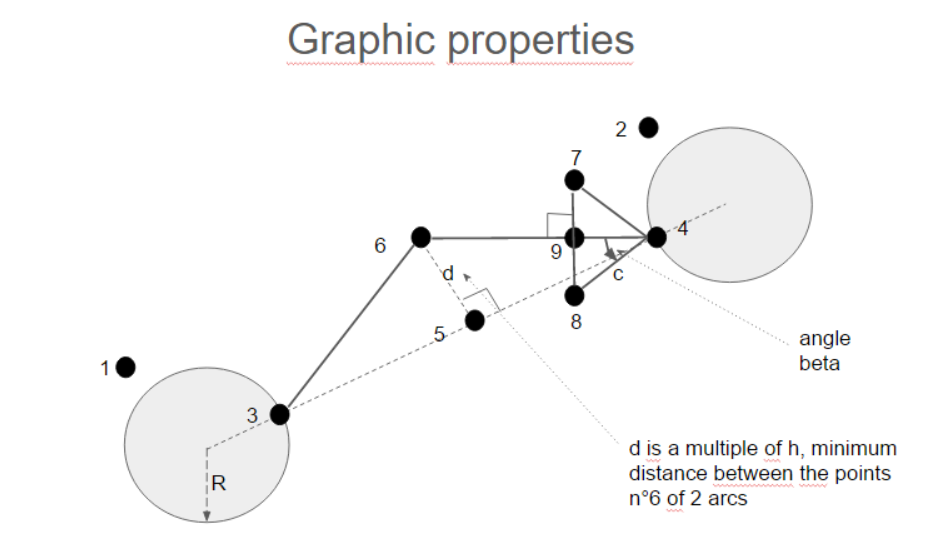
\includegraphics[width=17cm]{figures/graphical_properties}
  \caption{Graphe}
  \label{fig:graphical_properties}
\end{figure}


Dans le cas ou les noeuds 1 et 2 sont le même, 3 et 4 sont à des points opposés du cercle et l’arc est entre les deux (à l’intérieur du noeud). Celà permets d’éviter des conflits avec les arcs à l’extérieur. Nous avons renoncé à le mettre à l’extérieur car celà aurait été extrêmement lourd en calculs et nous aurait pris plusieurs jours, sans ajouter de fonctionnalité particulière.

Couleurs: nous avons 7 couleurs de base. Si l’utilisateur en ajoute une, elle sera générée automatiquement en fonction de l’algorithme suivant:
-génération d’une couleur aléatoire
-vérification d’une distance minimale avec les autres couleurs et le rouge (utilisé par le programme)
-acceptation ou nouvelle couleur aléatoire
Au bout d’un grand nombre d’itérations sans trouver, le programme surchargeait la mémoire, avec des effets destructeurs. Pour éviter celà, la distance minimale est réduite au bout d’un grand nombre d’itérations. Nous avons testé jusqu’à 70 couleurs.

\clearpage

\section{Démonstration de l'application}

Voici comment fonctionne notre application à l’utilisation sur notre figure~\ref{fig:utilisation_application}

\begin{figure}[h]
  \centering
  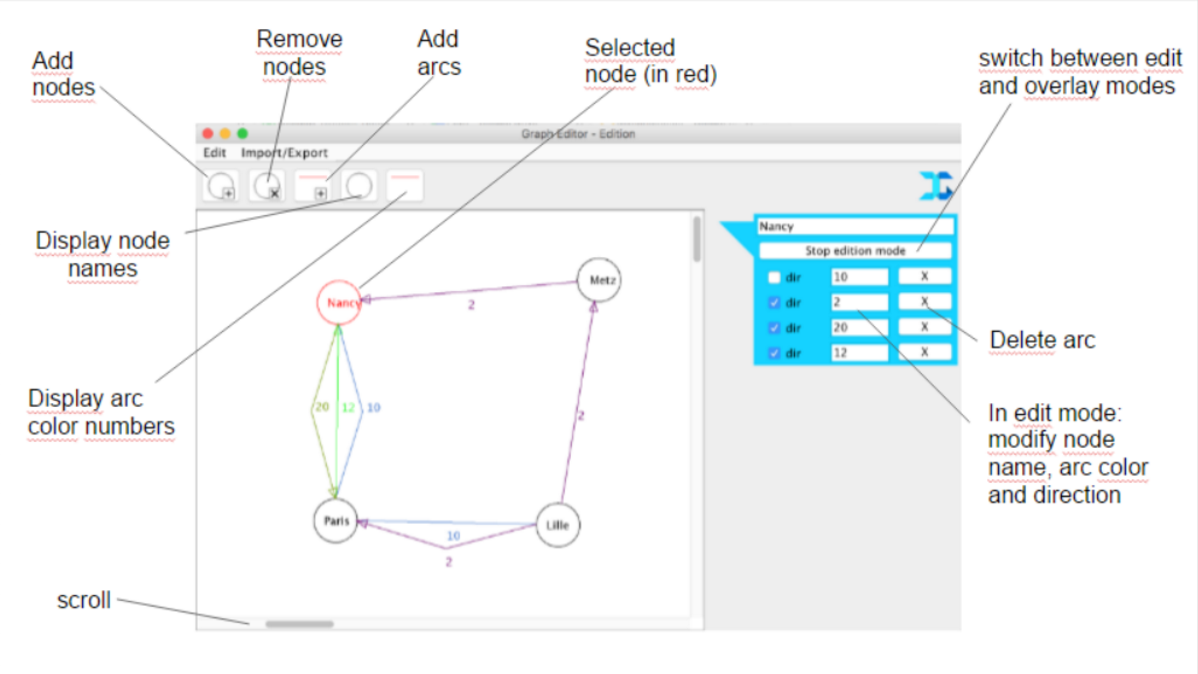
\includegraphics[width=17cm]{figures/exemples/utilisation_application}
  \caption{Exemple d'utilisation}
  \label{fig:utilisation_application}
\end{figure}

Une notice utilisateur se trouve en annexe.

Appuyer sur le bouton add node, add arc ou remove node active le bouton et permets de créer/supprimer plusieurs composants de suite. Créer un noeud requiert d’appuyer sur l’endroit ou l’on souhaite le créer, et créer un arc demande un click gauche sur l’origine et un click droit sur la destination (figure~\ref{fig:add_arc}).

\begin{figure}[h]
  \centering
  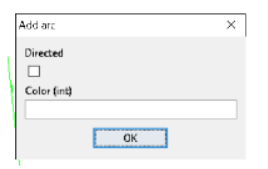
\includegraphics[width=5cm]{figures/exemples/add_arc}
  \caption{Ajout d'un arc}
  \label{fig:add_arc}
\end{figure}

Appuyer sur un noeud ouvre le menu de droite qui permets de voir ses arcs et de les supprimer. Passer la souris sur la description d’un arc le colorie en rouge pour l’identifier. En appuyant sur le bouton Edit, l’on peut modifier les propriétés du noeud et de ses arcs.
Dans le menu, l’on peut: 

\begin{itemize}
\item changer le nom du graphe - très utile avant un export vu que le nom du fichier généré dépends de celui du graphe.
\item importer ou exporter le graphe
\item accéder à la documentation
\item modifier une couleur (figure~\ref{fig:edit_color})
\end{itemize}


\begin{figure}[h]
  \centering
  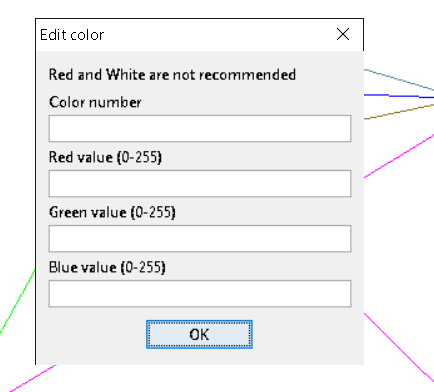
\includegraphics[width=10cm]{figures/exemples/edit_color}
  \caption{Edition d'une couleur}
  \label{fig:edit_color}
\end{figure}

Exemple d’utilisation: 
Notre encadrant nous avait donné deux graphes à transformer, voici pour le graphe 2 :

Sa représentation dans le pdf : figure~\ref{fig:graph2pdf}

\begin{figure}[h]
  \centering
  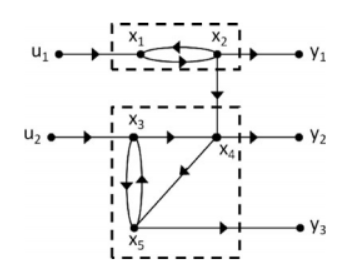
\includegraphics[width=10cm]{figures/exemples/graph2pdf}
  \caption{Graphe 2 depuis le pdf}
  \label{fig:graph2pdf}
\end{figure}

Sa reproduction dans l’application:  figure~\ref{fig:graph2App}

\begin{figure}[h]
  \centering
  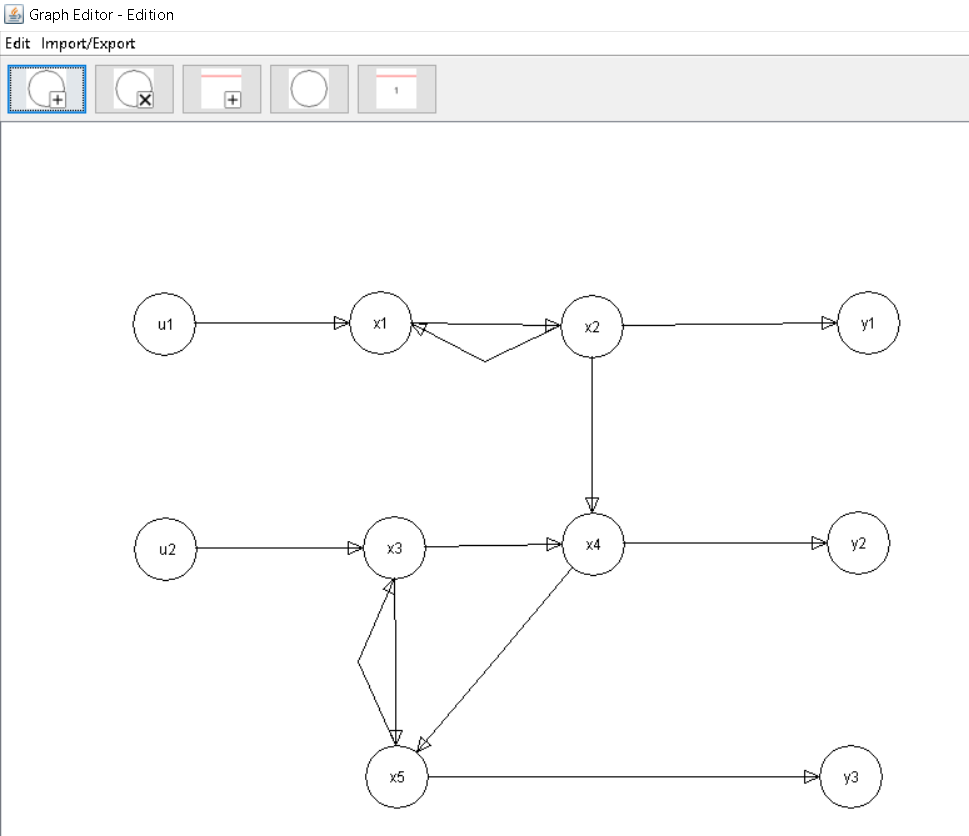
\includegraphics[width=10cm]{figures/exemples/graph2App}
  \caption{Graphe 2 depuis notre application}
  \label{fig:graph2App}
\end{figure}

Et ses matrices dans matlab: figure~\ref{fig:graph2Matlab}

\begin{figure}[h]
  \centering
  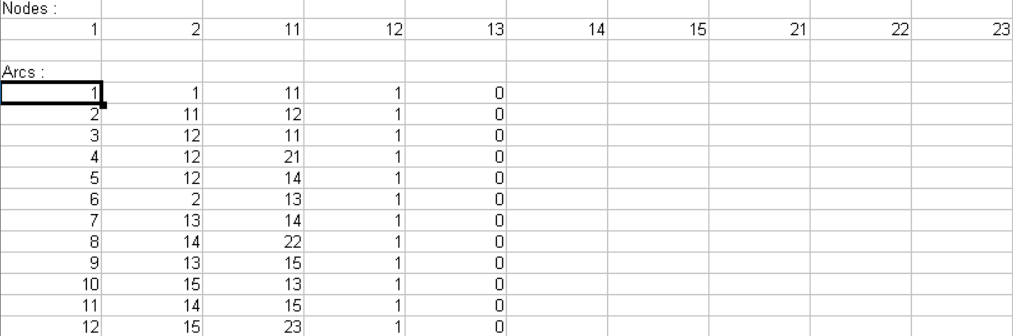
\includegraphics[width=10cm]{figures/exemples/graph2Matlab}
  \caption{Graphe 2 - Matrice sous matlab}
  \label{fig:graph2Matlab}
\end{figure}

\cleardoublepage

\chapter{Conclusion}

Nous sommes très satisfaits de notre travail. Nous avons répondu aux exigences formulées à chaque réunion avec notre encadrant et la synergie de groupe était parfaite.
L’application permet de gérer tout graphe (même si un graphe de plus de quelques centaines de noeuds risque de devenir peu illisible): il est possible de créer un graphe de bout en bout, modifier à souhait les noeuds et arcs, et sauvegarder son travail pour une séance future. 

De plus, notre code est très bien structuré et correctement commenté, permettant à de futurs développeurs d’apporter des nouvelles fonctionnalités, comme par exemple:

\begin{itemize}
\item Au niveau visuel, utiliser des arcs arrondis et si leur nombre est pair ne pas mettre un arc au milieu.
\item Afficher que des arcs d’une certaine couleur.
\item Mettre en place un algorithme créant une disposition des noeuds en fonction de leurs nombre et leurs arcs afin de gagner du temps.
\item Il serait possible plutôt que se connecter à matlab de le connecter à un autre programme en en ajoutant seulement un manager spécifique implémentant notre “IManagerConnector”.
\item Lors du chargement  d’un graphe, pouvoir rechercher dans les dossiers
\end{itemize}

Nous pouvons conclure que dans l’ensemble, le projet est une franche réussite et laisse la porte ouverte à de nombreuses améliorations.

\cleardoublepage

\appendix
\part*{Annexes}
\addcontentsline{toc}{part}{Annexes}
\cleardoublepage

\chapter{Code matlab de dynGraph.m}


\begin{lstlisting}[language=matlab, caption={dynGraph.m}, label={lst:dynGraph_m}]
classdef dynGraph < handle
    %GRAPH This is the class for creating and managing a dynamic graph editor for Matlab 
    %do not confuse with graph() from matlab code.
    
    properties
        nodes = [];
        arcs = [];
    end
    
    methods
        
        function out = varname(var)
            out = inputname(1);
        end
        
        %Placeholder: G's name should be aquired automatically.
        function G = draw(G,name)
            path = which('dynGraph');
            path = strrep(path, '.m', '.jar');
            javaaddpath(path);
            savepath
            javaObjectEDT('pidr.app.Application', name);
        end
        
        % To add multiple nodes, enter G = G.addNode(arrayOfNodes[])
        % If a single node can not be added, no nodes will be
        function G = addNode(G, nodeID)
            if size(G.nodes) > 0
                for c = nodeID 
                    if any(G.nodes == c)
                        error('Node with ID %d already exists\n', c);
                    end
                end
            end
            G.nodes = [G.nodes, nodeID];
            fprintf('Node added\n');
        end
        
        % To remove multiple nodes, enter G.removeNode(arrayOfNodes[])
        % If a single node can not be removed, no nodes will be
        function G = removeNode(G, nodeID)
            if size(G.nodes) > 0
                for c = nodeID 
                    if ~any(G.nodes == c)
                        error('Node with ID %d does not exist\n', c);
                    end
                end
            end
            for c = nodeID
                pos = find(G.nodes == c);
                G.nodes(pos) = [];
                if size(G.arcs) > 0
                    pos2 = [find(G.arcs(:,2) == c) ; find(G.arcs(:,3)== c)];
                    delete = G.arcs(pos2,1);
                    G.removeArc(delete);
                end
                fprintf('Node %d removed\n', c);
            end
        end
  
        
        % NodeID1 is the head of the arrow if directed equals 1
        % Directed and colorID are optional and set to 0 (not directed, black) by default
        % To add multiple arcs, the arguments must be columns
        % If a single arc can not be added, none will be
        % nodes at the head and tail of the arrow must exist
        function G = addArc(G, arcID, nodeID1, nodeID2, directed, colorID)
            s = size(arcID);
            uniqueID = unique(arcID);
            sU = size(uniqueID);
            
            if ~(sU(1) == s(1))
                error('two arcs with the same ID in parameters\n')
            end

            if nargin < 5
                directed = zeros(s(1),1);
            end
            
            if nargin < 6
                colorID = zeros(s(1),1);
            end
            
            if max(directed) > 1
                error('directed must be boolean (0 or 1)\n')
            end
            
            for c = nodeID1.'
                if ~any(G.nodes(1,:) == c)
                    error('head node %d does not exist\n', c)
                end
            end
            
            for c = nodeID2.'
                if ~any(G.nodes(1,:) == c)
                    error('tail node %d does not exist\n', c)
                end
            end
            
            for c = arcID.' 
                if size(G.arcs) > 0 
                    if any(G.arcs(:,1) == c)
                        error('Arc with ID %d already exists\n', c);
                    end
                end
            end
            G.arcs = [G.arcs; arcID, nodeID1, nodeID2, directed, colorID];
            fprintf('Arc added\n');
        end
        
        %This uses an arc matrix of the same format as arcs[] and tries to 
        %add the arcs in arcs[]. See addArc() description for more.
        function G = addArcs(G, arcMatrix, int)
            M = arcMatrix;
            [s1, s2] = size(M);
            if s2 > 5
                M = vec2mat(M,int);
                M = M.';
                [s1, s2] = size(M);
            end
            if 3 <= s2 && s2 <= 5
                if s2 == 3
                    M = [M, zeros(s(1),1)];
                end
                if s2 <= 4
                    M = [M, zeros(s(1),1)];
                end
                G.addArc(M(:,1),M(:,2),M(:,3),M(:,4),M(:,5))
            else
                error('arcMatrix must have between 3 and 5 columns\n')
            end
        end
        
        % To remove multiple arcs, the arguments must be a column
        % If said column contains the same ID multiple times, only one 
        % arc will be deleted, even if the method prints multiple lines
        % If a single arc can not be added, none will be
        function G = removeArc(G, arcID)
            if size(G.arcs) > 0
                for c = arcID.'
                    if ~any(G.arcs(:,1) == c)
                        error('Arc with ID %d does not exist\n', c);
                    end
                end
            end
            for c = arcID.'
                pos = find(G.arcs(:,1) == c);
                G.arcs(pos,:) = [];
                fprintf('Arc %d removed\n', c);
            end
        end
             
        function [G, nodes, arcs] = extract(G)
            nodes = G.arcs;
            arcs = G.nodes;
        end
        
        function G = clearArcs(G)
            G.arcs = [];
        end
        
        function G = clearNodes(G)
            G.nodes = [];
        end
        
        function G = clearAll(G)
            G.clearArcs();
            G.clearNodes();
        end
        
    end
    
    
end
\end{lstlisting}

\clearpage

\chapter{Manuel d'utilisateur - User Manual}

Welcome to the user manual for DynGraph.

\section{Launch}

Please refer to install.txt for the installation.
To launch the program, create a dynGraph name1
Then write in the command line name1.draw(‘name2’), where name2 is the name of another dynGraph (usually you want it to be name1 - but a typo can make you open another one).
This will launch the program and load the graph name2.

Note that ‘Test’ and ‘tmp’ are not supported graph names since both are used differently by the program and will be overwritten.


\section{Export/Import/Rename}

In the menu you will find and import/export menu and rename under “edit”. This will save your graph, the position of nodes and your custom colors.

To export a graph, you might want to rename it first. To do so simply click on “rename” and write the name you want. This will create a dynGraph in your workspace with the new name and the old data.

Then export it. This will create a name.csv file in your current folder, where name is the graphs’ name.

To import a graph, select the folder where its’ .csv file lies as the current folder. Then click on import and write the Graph’s name.

\section{Edit graph} 

Note: if clicking doesn’t seem to work, try making sure you don’t drag the mouse.

This is an image from the window:

\begin{figure}[h]
  \centering
  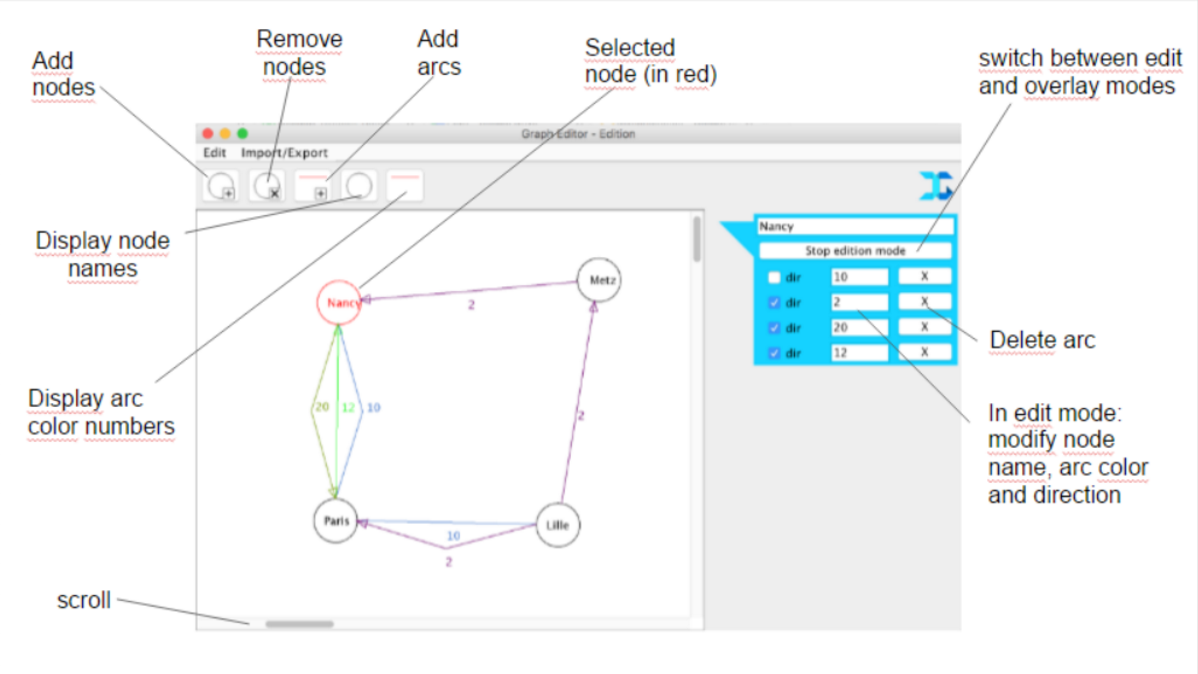
\includegraphics[width=17cm]{figures/exemples/utilisation_application}
  \caption{Exemple d'utilisation}
  \label{fig:utilisation_application}
\end{figure}

\underline{MOVE NODE :}
To move a node, click and drag it.

\underline{ADD NODE :} 
Toggle the add nodes button, then click where you want to create a node, then choose its’ name. Names need not be unique.

\underline{DELETE NODE :}
Toggle the delete nodes button then click on the nodes to remove them and any connected arc.

\underline{ADD ARC :}
Toggle the add arc button. Then click on the head node and right-click on the tail node. You must specify whever it is directed or not (default : not) and the color.

\underline{DELETE ARC :}
Click on a node to make connected arcs appear in a right-hand panel. Pass the mouse over them to color them in red. You can click on the cross near the arc  to delete them.

\underline{EDIT NODE/ARC :}
Select the node or a node connected to the arc. Then double click in the right-hand menu on the name of the node to switch to edit mode. This will toggle text fields : you can edit the name of the node, whether an arc is directed and it’s color. You can return to overlay mode by clicking on the button.

\underline{EDIT COLOR :}
Colors 0 through 7 have default values. Modifiying them is possible but won’t be saved in your export file.
Also, do not create a red color since it is used by the application for overlays.
Click on “edit” in the menu, and select edit color. Then write the number of the color you wish to edit or create, and its’ rgb values.

\section{Display}


\underline{DISPLAY NODE NAMES :}
Toggle the button to toggle the display of node names. If they are not displayed, moving your mouse over a node display its’ name under it.

\underline{DISPLAY ARC COLOR NUMBERS :}
Toggle the button to toggle the display of arc color numbers.

\cleardoublepage

\end{document}